% (c) 2002 Matthew Boedicker <mboedick@mboedick.org> (original author) http://mboedick.org
% (c) 2003-2007 David J. Grant <davidgrant-at-gmail.com> http://www.davidgrant.ca
% (c) 2008 Nathaniel Johnston <nathaniel@nathanieljohnston.com> http://www.nathanieljohnston.com
% (c) 2011 Scott Clark <sc932@cornell.edu> http://cam.cornell.edu/~sc932
% (c) 2015 Arne Hassel <arne.hassel@gmail.com> http://icanhasweb.net
%
% This work is licensed under the Creative Commons Attribution-Noncommercial-Share Alike 2.5 License. To view a copy of this license, visit
% http://creativecommons.org/licenses/by-nc-sa/2.5/ or send a letter to Creative Commons, 543 Howard Street, 5th Floor, San Francisco, California, 94105, USA.

\documentclass[letterpaper,10pt,english]{article}
\newlength{\outerbordwidth}
\pagestyle{empty}
\raggedbottom
\raggedright
\usepackage{babel}
\usepackage{float}
\usepackage[T1]{fontenc}
\usepackage{framed}
\usepackage{gfsartemisia-euler}
\usepackage{graphicx}
\usepackage{hyperref}
\usepackage[utf8]{inputenc}
\usepackage{tabularx}
\usepackage{tocloft}
\usepackage{url}
\usepackage[svgnames]{xcolor}
\usepackage{wrapfig}

%-----------------------------------------------------------

% Edit these values as you see fit

\setlength{\outerbordwidth}{2pt}  % Width of border outside of title bars
\definecolor{shadecolor}{gray}{0.75}  % Outer background color of title bars (0 = black, 1 = white)
\definecolor{shadecolorB}{gray}{0.93}  % Inner background color of title bars}

%-----------------------------------------------------------

% Margin setup

\setlength{\evensidemargin}{-0.25in}
\setlength{\headheight}{-0.25in}
\setlength{\headsep}{0in}
\setlength{\oddsidemargin}{-0.25in}
\setlength{\paperheight}{11in}
\setlength{\paperwidth}{8.5in}
\setlength{\tabcolsep}{0in}
\setlength{\textheight}{9in}
\setlength{\textwidth}{7in}
\setlength{\topmargin}{0in}
\setlength{\topskip}{0in}
\setlength{\voffset}{0.1in}

%-----------------------------------------------------------

% Custom commands

\newcommand{\resitem}[1]{\item #1 \vspace{-2pt}}

\newcommand{\resheading}[1]{\vspace{8pt}
\parbox{\textwidth}{\setlength{\FrameSep}{\outerbordwidth}
  \begin{shaded}
    \setlength{\fboxsep}{0pt}\framebox[\textwidth][l]{\setlength{\fboxsep}{4pt}\fcolorbox{shadecolorB}{shadecolorB}{\textbf{\sffamily{\mbox{~}\makebox[6.762in][l]{\large #1} \vphantom{p\^{E}}}}}}
  \end{shaded}
}\vspace{-5pt}
}

\newcommand{\ressubheading}[4]{
  \begin{tabularx}{6.5in}{l@{\cftdotfill{\cftsecdotsep}\extracolsep{\fill}}r}
    \textbf{#1} & #2          \\
    \textit{#3} & \textit{#4} \\
  \end{tabularx}\vspace{-6pt}}

%-----------------------------------------------------------

\title{Curriculum Vitae}

\begin{document}

  \begin{minipage}{\textwidth}
    \begin{wrapfigure}{r}{0pt}
      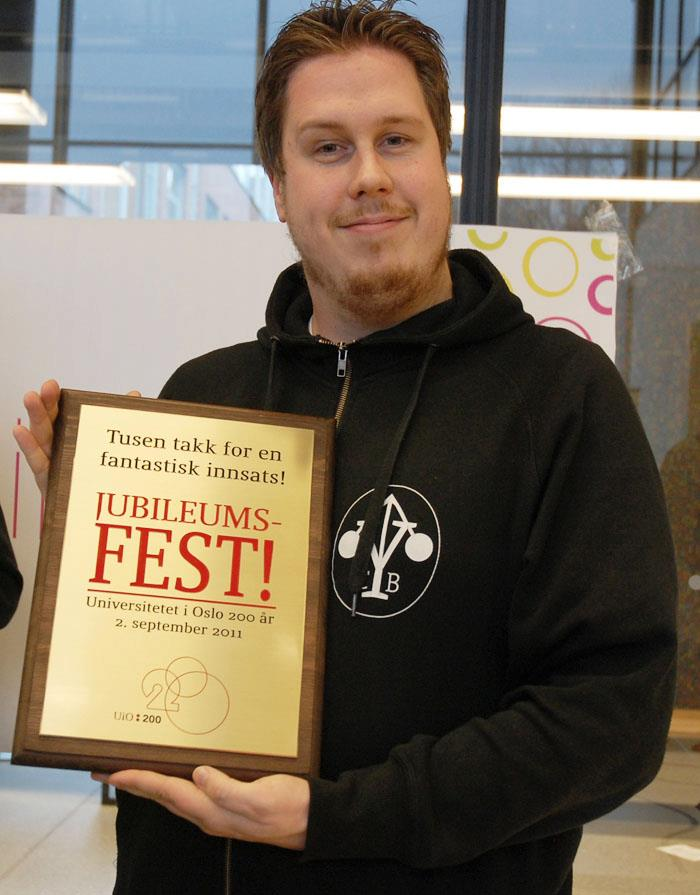
\includegraphics[height=45mm]{uio200.jpg}
    \end{wrapfigure}

    \textbf{\Large Curriculum Vitae for Arne Hassel}

    \vspace{5mm}

    \begin{tabular}{p{1in} l}
      Adress:         & Helgesens gate 12 F, 0553 Oslo, NORWAY \\
      Phone:          & (+47) 416 94 086                       \\
      Mail:           & \url{arne.hassel@gmail.com}            \\
      Born:           & December 5th 1984                      \\
      Marital status: & Unmarried                              \\
    \end{tabular}

    \vspace{5mm}

    \begin{minipage}{5.5in}
      Highly experienced front-end programmer with a master in computer science and bachelor in economics. I love to work with web-based technologies such as
      HTML, CSS, TypeScript and \href{https://www.w3.org/standards/semanticweb/data}{Linked Data}. I'm a great team player and strive to make sure that all
      applications that I work on are accessible and respectful of all user groups. I'm also a strong believer in the power that Linked Data can unleash for
      services and end-users. I've enjoyed working as a mentor for less experienced developers, and have been credited for my patience and ability to answer
      questions.
    \end{minipage}

  \end{minipage}

  \resheading{Work Experience}

  \begin{itemize}
    \item
    \ressubheading{Inrupt}{Oslo}{Senior front-end developer}{2018 - 2022}
    \begin{itemize}
      \item Worked on several projects related to
      \href{https://solidproject.org/}{the Solid project} where I had the honour of working with
      \href{https://en.wikipedia.org/wiki/Tim_Berners-Lee}{Tim Berners-Lee}. Also worked a lot with React.
    \end{itemize}
    \item
    \ressubheading{Bouvet ASA}{Oslo}{Senior front-end developer}{2017 - 2019}
    \begin{itemize}
      \item Worked with Tine and Arkivverket as front-end tech lead, using
      \href{https://enonic.com/resources/enonic-xp-all-you-need-to-know}{Enonic XP} and React.
    \end{itemize}
    \item
    \ressubheading{Questback AS}{Oslo}{Front-end developer}{2014 - 2017}
    \begin{itemize}
      \item Responsible for the front-end development on Questback Essentials, the DIY survey tool created and developed by Questback.
    \end{itemize}
    \item
    \ressubheading{Centre for Shared Decision making and Collaborative Care Research}{Oslo, Norway}{System developer}{2008 - 2014}
    \begin{itemize}
      \resitem{Worked mostly frontend (HTML, CSS og Javascript), but also some backend (.NET)}
    \end{itemize}
    \item
    \ressubheading{Senter for Helse \& Arbeid}{Oslo, Norway}{Personal assistant}{2008}
    \item
    \ressubheading{Kiwi}{Risør \& Oslo, Norway}{Part-time worker}{1999 - 2008}
  \end{itemize}

  \resheading{Education}
  \begin{itemize}
    \item
    \ressubheading{Department of informatics, University of Oslo}{Oslo, Norway}{Master of Computer Science: programming and networks (current)}{2010 - 2012}
    \begin{itemize}
      \item Wrote my master thesis on Javascript and Semantic Web. My supervisors were Kjetil Kjernsmo and Martin Giese.
    \end{itemize}
    \item
    \ressubheading{Department of informatics, University of Oslo}{Oslo, Norway}{5-year Master, Distributed Systems and Networks}{2007 -2010}
    \item
    \ressubheading{Norwegian University of Life Sciences}{Ås, Norway}{Bachelor in Economics and Administration}{2003 - 2007}
    \item
    \ressubheading{Risør VGS}{Risør, Norway}{General studies}{2000 - 2003}
  \end{itemize}

  \resheading{Skills \& Certifications}

  See attached competence chart for more details.

  \begin{itemize}
    \item MS: Programming in HTML5 with JavaScript and CSS3 (Microsoft, 2015)
    \item MCPS: Microsoft Certified Professional (Microsoft, 2015)
    \item Certified ScrumMaster (Scrum Alliance, 2013-2015)
  \end{itemize}

  \resheading{Selected projects}

  \begin{itemize}
    \item {\bf Ifi-ordenen webpage:} Webpage developed with \href{https://nextjs.org/}{Next}/React and \href{https://www.sanity.io/}{Sanity}. Collaborated
    with designers to make sure it's optimized for students.
    \url{https://ordenen.ifi.uio.no/}
    \item {\bf CYB50 webpage:} Published the anniversary book that I was editor for. Used \href{https://www.gatsbyjs.com/}{Gatsby}/React and MDX-files for
    content.
    \url{https://50.cyb.no/}
  \end{itemize}

  \resheading{Voluntary Work and Honorary Positions}

  \begin{itemize}
    \item
    \ressubheading{Solid}{Oslo}{Volunteer}{2018 - current}
    \item
    \ressubheading{CYB50 Anniversary Book}{Oslo}{Editor}{2018-2019}
    \item
    \ressubheading{Hennes Majestet Keiserpingvinen den Fornemmes orden}{Oslo}{Grand master}{2014 - current}
    \item
    \ressubheading{Holder de ord}{Oslo, Norway}{Web developer}{2012 - 2018}
    \item
    \ressubheading{Kodeklubben Oslo}{Oslo, Norway}{Code supervisor}{2015 - 2016}
    \item
    \ressubheading{Cybernetic Society (CYB)}{Oslo, Norway}{Treasurer, Member of the Sponsor Board, Guard}{2009 - 2012}
    \item
    \ressubheading{Birthday Party at Ole-Johan Dahls hus September 2nd}{Oslo, Norway}{Party General/Coordinator (worked with University of Oslo)}{2011}
    \item
    \ressubheading{IAESTE}{Ås, Norway}{National Computer Manager, Leader, Treasurerer, Vice Leader}{2003 - 2007}
    \item
    \ressubheading{UKA i Ås}{Ås, Norway}{Webmaster, Guard}{2004, 2006}
  \end{itemize}

  \resheading{Personal details}

  \begin{itemize}
    \item {\bf Hobbies:} Reading, producing music
    \item Have a driver license class B (norwegian)
  \end{itemize}

\end{document}
